\documentclass[
	fontzize=12pt, % Fontsize
	paper=a4, % DIN format A4
	openany,	% starts the chapter on the next page (even or odd).
	bibliography=totoc % adds bib to table of contents
	]{scrbook}

% Include definitions, custom commands, packages and so on 
% ##################################################
% Document variables
% ##################################################

% Personal data of the author
\newcommand{\docSurnameA}{Berger}
\newcommand{\docPrenameA}{Adrian}
\newcommand{\docEmailA}{adrian.berger.2@students.bfh.ch}

% Data of the University
\newcommand{\docLocationFH}{Bern}
\newcommand{\docFieldOfStudy}{BSc Computer Science}


% Document data
\newcommand{\docTitle}{Data Mining}
\newcommand{\docSecondTitle}{Einführung und Beispiele}
\newcommand{\docKindOfWork}{IT-Seminar}
\newcommand{\docHandOverDate}{25.05.2021}
\newcommand{\docFirstLector}{Jürgen Eckerle}
\newcommand{\docModule}{BTI7311}

% Used for toggle-if case
\usepackage{etoolbox}

% Conditional variables
\providetoggle{useCode}
\settoggle{useCode}{false}
\providetoggle{useAbstract}
\settoggle{useAbstract}{true}

% ##################################################
% General packages
% ##################################################

\usepackage{cmap} % Make PDF files searchable and copyable
\usepackage[T1]{fontenc} % used for west European language support
\usepackage[utf8]{inputenc} % Allows usage of umlaute
\usepackage{multicol}

% Set language to english
\usepackage[german]{babel}

% Use graphics/pictures
\usepackage{graphicx}

% Colours (be able to define custom colours)
\usepackage{color}
\usepackage[usenames,dvipsnames,svgnames,table]{xcolor}

% Masking of URLs and file paths
\usepackage[hyphens]{url}

% Nice quotes
\usepackage{csquotes}

% Package for indexing (Schlagwortverzeichnis)
%\usepackage{index}
%\makeindex

% Ipsum Lorem
\usepackage{lipsum}


% ##################################################
% Page formatting
% ##################################################
\usepackage[
	inner=2.5cm, % Left margin
	outer=2.5cm, % Right marin
	top=1.5cm,   % Top marin
	bottom=2cm,  % Bottom marin
	includefoot, % Include footer to bottom margin
	includehead  % Include header to top margin
	]{geometry}

% ##################################################
% Header and footer
% ##################################################

\usepackage{fancyhdr}  % allows manipulation of header and footer

\pagestyle{fancy} % lets you define your own style
\fancyhf{}
\fancyhead[EL,OR]{\sffamily\thepage} % page number even=left, odd=right
\fancyhead[ER,OL]{\sffamily\nouppercase{\leftmark}} % chapter even=left, odd=right
\fancyfoot[LE,LO]{Berner Fachhochschule}
\fancyfoot[RE,RO]{\docPrenameA~\docSurnameA}


\renewcommand{\footrulewidth}{1pt}		% add footer line by setting it to one

\fancypagestyle{headings}{}
\fancypagestyle{plain}{}

% No header/footer on empty pages
\fancypagestyle{empty}{
  \fancyhf{}
  \renewcommand{\headrulewidth}{0pt}
  \renewcommand{\footrulewidth}{0pt}
}


%Saves \chaptermark in \oldchaptermark so that 
% it can be reset for the appendix
\let\oldchaptermark\chaptermark

%No "Chapter # NAME" in header
\renewcommand{\chaptermark}[1]{
	\markboth{#1}{}
   	\markboth{\thechapter.\ #1}{}
}

% ##################################################
% fonts
% ##################################################

% Set default font
\renewcommand{\familydefault}{\sfdefault}

% Set default line distance to 1.5
\usepackage{setspace}
\onehalfspacing 

% Set font size
\addtokomafont{chapter}{\sffamily\Large\bfseries} 
\addtokomafont{section}{\sffamily\large\bfseries} 
\addtokomafont{subsection}{\sffamily\normalsize\bfseries} 
\addtokomafont{caption}{\sffamily\normalsize\mdseries} 

%Disable indent of paragraphs
\setlength{\parindent}{0pt}

%Line distances of paragraphs
\usepackage{parskip}

% ##################################################
% Table of contents / General listings
% ##################################################

% Control table of contents, figures
\usepackage{tocloft}

% Points also for chapters
\renewcommand{\cftchapdotsep}{3}
\renewcommand{\cftdotsep}{3}

% Adjust font and size in table of contents
\renewcommand{\cftchapfont}{\sffamily\normalsize}
\renewcommand{\cftsecfont}{\sffamily\normalsize}
\renewcommand{\cftsubsecfont}{\sffamily\normalsize}
\renewcommand{\cftchappagefont}{\sffamily\normalsize}
\renewcommand{\cftsecpagefont}{\sffamily\normalsize}
\renewcommand{\cftsubsecpagefont}{\sffamily\normalsize}

%Set space between lines in listings
\setlength{\cftparskip}{.5\baselineskip}
\setlength{\cftbeforechapskip}{.1\baselineskip}


% ##################################################
% List of tables and tables
% ##################################################

% Numbering of tables
\renewcommand{\thetable}{\arabic{table}}
\counterwithout{table}{chapter}

% Adjust list of tables
\renewcommand{\cfttabpresnum}{Table }
\renewcommand{\cfttabaftersnum}{:}

% Width of numbering scope [Table 1:]
\newlength{\tableLength}
\settowidth{\tableLength}{\bfseries\cfttabpresnum\cfttabaftersnum}
\addtolength{\tableLength}{3mm} %extra offset
\setlength{\cfttabnumwidth}{\tableLength}
\setlength{\cfttabindent}{0cm}

%Adjust font
\renewcommand\cfttabfont{\sffamily}
\renewcommand\cfttabpagefont{\sffamily}

% Suppress vertical lines
\usepackage{booktabs}

%Multi row for specific rows
\usepackage{multirow}

%Additional table package
\usepackage{tabu}

% ##################################################
% Table of figures and figures
% ##################################################

\usepackage{caption}

\usepackage{wrapfig}

% Numbering of figures
\renewcommand{\thefigure}{\arabic{figure}}
\usepackage{chngcntr}
\counterwithout{figure}{chapter}

% Adjust table of figures
\renewcommand{\cftfigpresnum}{Figure }
\renewcommand{\cftfigaftersnum}{:}

% Width of numbering scope [Figure 1:]
\newlength{\figureLength}
\settowidth{\figureLength}{\bfseries\cftfigpresnum\cftfigaftersnum}
\addtolength{\figureLength}{2mm} %extra offset
\setlength{\cftfignumwidth}{\figureLength}
\setlength{\cftfigindent}{0cm}

% Adjust font
\renewcommand\cftfigfont{\sffamily}
\renewcommand\cftfigpagefont{\sffamily}

%Default paths
\graphicspath{ {./content/pictures/} }


% ##################################################
% Appendix
% ##################################################

%Calc packet for calculations
\usepackage{calc}
\usepackage{amsmath}

%Appendix packet, set the flags for the TOC
\usepackage[toc,title,titletoc]{appendix} 


% Change text for title
%\renewcommand{\appendixtocname}{Appendix}

%Befehl für einen neuen Bericht und die erste Seite als Bild
\newcommand{\appendixsection}[2]{
\section{#1}
\appendixsingle{#2}
}

%Befehl für einzelne Seite als Bild eingefasst, damit Überschrift und Kopfzeile
% bestehen bleibt. 
\newcommand{\appendixsingle}[1]{
\vspace{-10cm}
\vfill
\mbox{}\hspace{-1.5cm}\includegraphics[width=\linewidth+3cm]{#1}\hspace{-1.5cm}\mbox{}
\vspace{-10cm}
\vfill
\mbox{}
}

%Datenträger Tabelle
\definecolor{lightgray}{gray}{0.85}
\definecolor{ultralightgray}{gray}{0.95}
\definecolor{mygray}{gray}{0.70}

% ##################################################
% Theoreme
% ##################################################

% Umgebung fuer Beispiele
%\newtheorem{beispiel}{Beispiel}

% Umgebung fuer These
%\newtheorem{these}{These}

% Umgebung fuer Definitionen
%\newtheorem{definition}{Definition}
  	
% ##################################################
% Literaturverzeichnis
% ##################################################
\usepackage{biblatex}
\bibliography{sample} % file to use (without .bib)
%\bibliographystyle{alpha} % set style of bibliography

% ##################################################
% Abkuerzungsverzeichnis
% ##################################################

\usepackage{acronym}

% ##################################################
% PDF / Dokumenteninternelinks
% ##################################################

\usepackage[
	colorlinks=false,
   	linkcolor=black,
   	citecolor=black,
  	filecolor=black,
	urlcolor=black,
    bookmarks=true,
    bookmarksopen=true,
    bookmarksopenlevel=3,
    bookmarksnumbered,
    plainpages=false,
    pdfpagelabels=true,
    hyperfootnotes,
    hidelinks,
    pdftitle ={\docTitle},
    pdfauthor={\docPrenameA~\docSurnameA},
    pdfcreator={\docPrenameA~\docSurnameA}]{hyperref}




% Start of the document
\begin{document}

\setcounter{secnumdepth}{3}

% Titelblatt
\begin{titlepage}
\pagestyle{empty}

% ##################################################
% BFH-Logo einbinden
% ##################################################
\begin{flushleft}
\begin{figure}[ht]
\flushleft

\includegraphics[height=3cm]{content/pictures/bfh_logo.jpeg}
\end{figure}
\end{flushleft}

% ##################################################
% Titel
% ##################################################
\begin{center}
{\fontsize{18}{22} \selectfont \docKindOfWork}\\[5mm]
{\fontsize{18}{22} \selectfont im Studiengang} \\[5mm]
{\fontsize{18}{22} \selectfont \docFieldOfStudy}\\
\vspace{1cm}

\begin{onehalfspace}
{\fontsize{32}{24} \selectfont \docTitle}\\[7mm]
{\fontsize{18}{22} \selectfont \docSecondTitle}

\end{onehalfspace}
\end{center}

\begin{figure}[h!]
	\centering
	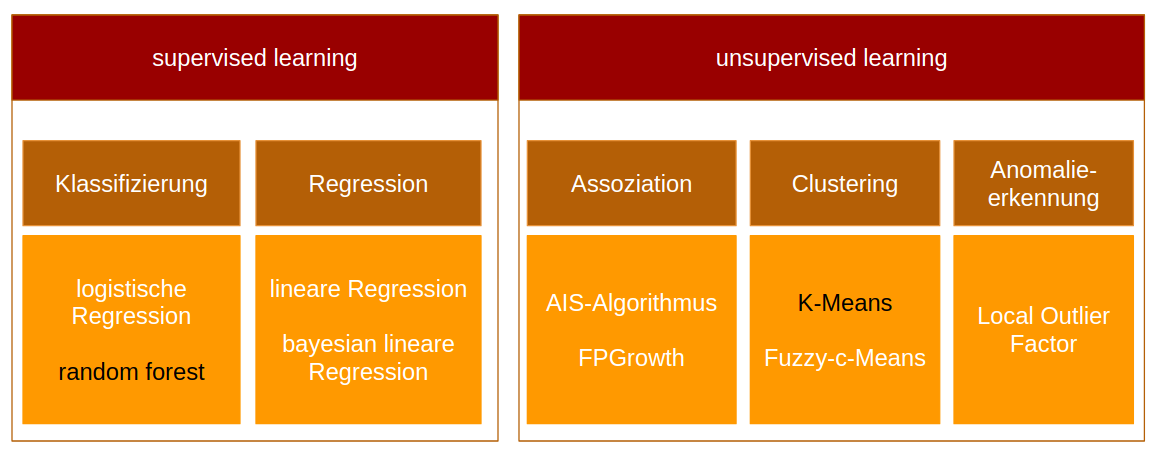
\includegraphics[width=1\textwidth]{verfahren.png}
\end{figure}

% ##################################################
% Zusatzinformationen
% ##################################################
\vfill
\begin{center}
\begin{tabular}{lcl}
Verfasser	 	&:& \docPrenameA~\docSurnameA\\
				& & \docEmailA 	\\ \\
Dozent  		&:& \docFirstLector 	\\ \\
Modul	  		&:& \docModule 	\\ \\
Datum			&:& \docHandOverDate 	\\ \\

					
\end{tabular}
\end{center}
\end{titlepage}

\pagenumbering{Roman}

\iftoggle{useAbstract}{
	% Abstract
	\chapter*{Abstract\markboth{Abstract}{}}
Diese Arbeit bietet einen Überblick über die Thematiken im Bereich Data Mining. Dazu werden einleitend Beispiele vorgestellt, bei welchen Data Mining verwendet wurde. Hierbei handelt es sich einerseits um Beispiele aus dem Bereich Gesundheit, Sicherheit, Landwirtschaft sowie ein kommerzielles Beispiel.
Zudem wird in der Arbeit eine kurze Übersicht zu den ethischen Überlegungen und Bedenken gegeben.
Der Hauptteil der Arbeit beschäftigt sich mit den verschiedenen Verfahren im Bereich Data Mining und Machine Learning.

Dabei soll eine Übersicht über die Verfahren, sowie die wichtigsten Stichwörter dazu gegeben werden. Diese Übersicht soll es der Leserschaft ermöglichen einen Überblick zu den Verfahren zu erhalten, aber auch gezielt weiterführende Themen ansprechen. Somit soll die Leserschaft gezielt motiviert werden, die weiterführenden Themen nach eigenen Interessen durch die referenzierten Dokumente zu vertiefen.

Gegen Ende des Dokumentes werden konkret die Verfahren Random Forest und K-means vorgestellt. Diese dienen beispielhaft dazu, die Komplexität des Data Mining aufzuzeigen. Auch hier werden gezielt Stichwörter eingesetzt, welche die Leserschaft für eigene, weitere Recherchen verwenden kann.

}

% Inhaltsverzeichnis
\tableofcontents

\pagenumbering{arabic}
\RedeclareSectionCommand[beforeskip=10pt, afterskip=15pt]{chapter}
% Include chapters here:
\chapter{Einleitung}

\section{Definition}
Data Mining ist ein Sammelbegriff für die Anwendung statistischer Verfahren auf grosse Datenmengen. Das Ziel dieser Verfahren ist es, aus den Daten neue Erkenntnisse zu gewinnen, wie etwa Korrelationen oder Trends zu identifizieren. Durch die Anwendung von Data Mining können in grossen Datenmengen Muster und Regeln erkannt werden, die durch manuelle Auswertungen nur schwer zu erkennen sind.
Entgegen der möglichen Erwartung aus dem Begriff Data Mining, geht es bei diesen Verfahren nicht darum, Daten zu generieren oder zu sammeln. Dieser Prozessschritt geschieht jeweils vor dem Data Mining und ist somit nicht Teil vom Data Mining Prozess. \cite{definition}

\section{Erläuterungen}
Grundsätzlich beruht Data Mining meist auf Verfahren der Statistik und somit aufgrund mathematischer Grundlagen. In vielen Fällen beruhen diese statistischen Verfahren entweder auf statistischen Variabeln oder auf Zufallsvariablen, welche mittels Wahrscheinlichkeitsrechnungen bestimmt werden können. In vielen der aktuell verwendeten Verfahren werden mehrere dieser Variablen gleichzeitig untersucht. Dieses Vorgehen werden auch multivariate Verfahren genannt.

Häufig wird auch Machine Learning als Data Mining bezeichnet. Dies ist historisch aber nicht ganz korrekt. Während es beim Data Mining darum geht, neue Muster und somit Erkenntnisse aus Daten zu gewinnen, versucht man mit Machine Learning neue Berechnungsfunktionen aus den Daten abzuleiten. Moderne Data Mining Verfahren verwenden jedoch meist Techniken aus dem Bereich des Machine Learning. Im Folgenden werden Techniken und Verfahren gezeigt, die teilweise aus einer Überschneidung von Data Mining und Machine Learning bestehen. \cite{dmdefinition}

\clearpage
\section{Beispiele von Anwendungsfälle}
\subsection{Watson for Oncology}
Watson for Oncology (WFO) ist eine von IMB entwickelte Plattform, die bei der Behandlung von Krebspatienten helfen soll. Diese Plattform ist ein spannendes Beispiel dafür, wie Data Mining und Machine Learning den Menschen unterstützen kann, jedoch zeigt es auch, wo die Schwierigkeiten bei einem solchen System entstehen.

WFO wurde als Unterstützung für Ärzte*innen entwickelt, welche entscheiden, welche Krebsbehandlung eine krebskranke Person erhalten soll. Dabei kennt WFO eine vorgegebene Liste an Behandlungen. Aufgrund der Patientenakte entscheidet WFO anschliessend, welcher diese Behandlungen empfohlen werden können. WFO entwickelt also nicht eigenständig neue Behandlungen, sondern wählt aus bekannten Methoden die besten aus.

Diese Auswahl basiert auf den Informationen des Patientendossiers. Dies beinhaltet einerseits persönliche Merkmale wie das Alter oder das Geschlecht, aber auch die gesundheitlichen Informationen wie die Art und Stufe des Tumors, sowie die bereits durchgeführten Vorbehandlungen.
Diese Daten werden mit früheren Patientendaten verglichen, bei welchen die damals gewählte Methodik für die Behandlung bekannt ist. Aufgrund dieses Vergleichs schlägt WFO die besten Methoden vor und schliesst auch gewisse Methoden aus.

Das behandelnden Ärzteteam nutzen anschliessend dieses Resultat als weitere Hilfestellung bei der Entscheidung, welche Behandlungsmethode gewählt wird.
WFO trifft also nicht direkt eine Entscheidung, sondern dient lediglich als Hilfsmittel. Die effektive Behandlungsart wird aktuell immer von Ärzteteam ausgewählt.

Diverse Studien zu WFO haben ergeben, dass WFO als Hilfsmittel hilfreich sein kann, jedoch noch diverses Schwierigkeiten aufweist, bevor es die Evaluation eines Ärzteteams komplett ersetzen kann.

Das Hauptproblem dabei ist, dass WFO nicht vollständig transparent ist, aufgrund von welchen Informationen welche Behandlung vorgeschlagen wurde. 
Dies führt dazu, dass das Ärzteteam die Vorschläge nicht zwangsläufig nachvollziehen kann und allfällige Unstimmigkeiten im WFO-Algorithmus nicht erkannt werden können.

Ein weiteres Problem ist die Datengrundlage. WFO proklamiert eine Übereinstimmung von rund 93\% zwischen den von WFO vorgeschlagenen Behandlungen und den von Fachpersonen vorgeschlagenen Behandlungen.
Unabhängige Untersuchungen haben nun jedoch ergeben, dass dies stark davon abhängt, welche Art von Krebs vorliegt und in welcher Patientengruppe (Alter, Geschlecht) die zu behandelnde Person ist. \cite{wfo1} \cite{wfo2} \cite{wfo3}


\subsection{Netflix Thumbnails}
Sobald es um Gewinnung von Informationen aus Daten geht, wird oft Netflix genannt. Netflix hat sich in den letzten Jahren nicht zuletzt durch gesammelte Daten einen grossen Marktanteil im Online Streaming erarbeitet.
Dabei trackt Netflix seine Nutzenden und versucht aufgrund des Verhaltens dieser Nutzenden herauszufinden, wieso eine Person ein Film oder eine Serie konsumiert.\cite{netflix}

Anschliessend wird versucht, dieses Verhalten künstlich zu erzeugen. Das einfachste Beispiel dazu ist die Generierung der Thumbnails (Vorschaubilder). Je nach Präferenz der aktuell eingeloggten Person werden andere Bilder angezeigt. Im Rahmen dieser Arbeit wurde ein kleiner Selbsttest durchgeführt. Auf fünf verschiedenen Konten wurde nach der britischen Serie Peaky Blinders gesucht. Dabei wurden drei unterschiedliche Thumbnails angezeigt:
\begin{figure*}[ht!]
	
\includegraphics[width=.3\textwidth]{peakyblinders1.png}\hfill
	
\includegraphics[width=.3\textwidth]{peakyblinders2.png}\hfill
	
\includegraphics[width=.3\textwidth]{peakyblinders3.png}
	\caption{Angezeigte Thumbnails bei verschiedenene Netflix Konten (Quelle: Netflix)}
\end{figure*}

Das linke Bild wurde nur in einem Konto angezeigt, während das mittlere und das rechte jeweils in zwei der fünf Konten angezeigt wurden.
Spannend dabei ist das mittlere Bild. Eine der beiden Personen gab an, dass sie kürzlich eine Serie mit Anya Taylor-Joy (der Schauspielerin im Bild) geschaut hat. Die andere Person gab an, die Schauspielerin nicht zu kennen, nannte aber eine Vorliebe für Liebesdramen. Beides scheinen hier gute Gründe zu sein, dieses Thumbnail den anderen Thumbnails vorzuziehen. Die beiden Personen, welche das rechte Bild angezeigt erhielten, gaben an, allem voran Dramen und Thriller zu konsumieren, was das Thumbnail ebenfalls erklären könnte. Für das linke Bild konnte kein ausschlaggebendes Kriterium erkannt werden, da die Person keine spezifische Film-Vorliebe angeben konnte.

Obwohl hier über die Gründe nur gemutmasst werden kann, zeigt es doch, welche Kriterien Netflix für die Anzeige eines Thumbnails verwendet und wie dadurch die Aufmerksamkeit der Nutzenden geweckt werden soll.

\subsection{Erkennung von Verbrechensmustern}
Bereits 1949 veröffentlichte George Orwell das Buch mit dem Titel 1984. Dabei beschrieb er einen totalitären Überwachungsstaat, welcher fast die gesamte Privatsphäre seiner Bürger*innen unterdrückt. Dabei wird das Verhalten der einzelnen Personen überwacht und falsches, dem Staat nicht genehmes Verhalten bestraft. 
Dieser Ansatz wird heutzutage in gewissen Gebieten in die Wirklichkeit umgesetzt. Durch die Digitalisierung kann die Bevölkerung heute genauer untersucht und überwacht werden.
Ein Beispiel dazu ist die Erkennung von Verbrechensmustern. Dabei wird versucht in bekannten Verbrechensdaten Muster zu erkennen, die Aufschluss darüber geben sollen, wann und wo das nächste Verbrechen verübt werden soll.

Ein gutes Beispiel dazu ist das Chicago Police Department. Dieses wendet Data Mining Techniken auf polizeiliche Datensätze an, darunter Kriminalitätsvorfälle, Verhaftungen und Wetterdaten. Diese historischen Daten werden mit IoT-Echtzeitdaten kombiniert (z. B. mit sensorgesteuerten Kameras). Dadurch können Verbrechen zeitnah oder sogar vor der Ausübung erkannt werden.

Durch dieses Verfahren können auch Regionen erkannt werden, in welchen überdurchschnittlich viele Verbrechen verübt werden. Diese Regionen können anschliessend genauer überwacht und geprüft werden.
Wie Orwell bereits früh erkannt hat, führt dies auch zu diversen Nebeneffekten, die vielfach als Negativ aufgefasst werden. Auf einige davon wird im Kapitel \hyperref[sec:ethics]{Ethische Grundsätze} eingegangen.\cite{crime-prevention}

Ein einfaches Verfahren zur Gruppierung von Verbrechen in Regionen, Zeiteinheiten oder Verbrechensart ist das Clustering. Dieses wird im Kapitel \hyperref[sec:clustering]{Clusteranalyse} genauer erläutert. Dabei werden die bestehenden Verbrechen in Gruppen eingeteilt. Durch diese Gruppen können anschliessend Erkenntnisse gefunden werden, welche Regionen besonders gefährdet sind, oder welche Faktoren zu Verbrechen führen.\cite{crime}

Diese Art von Verbrechenserkennung hat durch die Digitalisierung stark zugenommen und es ist davon auszugehen, dass diese Analysen in Zukunft exakter und ausführlicher werden dürften.

\subsection{Bayer}
Ein kleines aber sehr spezifisches Beispiel für die Verwendung von Machine Learning und Data Mining ist die Unkrauterkennung der Firma Bayer.

Bayer hat über die Jahre rund 100'000 Bilder von Unkraut gesammelt. Daraus ergibt sich eine Datenbank von 70 Arten an Unkraut.
Damit ein Bauer nun das Unkraut möglichst effektiv vernichten kann, nutze er diese Datenbank als Grundlage. Er kann ein Foto des Unkrautes hochladen und erhält die Information, um welches Unkraut es sich handelt.

Dadurch können die Landwirte die Auswirkungen ihrer Entscheidungen – zum Beispiel die Wahl des Saatguts, die Menge an Pflanzenschutzmitteln oder den Erntezeitpunkt – viel genauer vorhersagen.\cite{bayer}

\clearpage
\section{Ethische Grundsätze}
\label{sec:ethics}
Grundsätzlich gibt es viele ethische Überlegungen zu klären, sobald aus Daten Informationen gewonnen werden sollen. Diese alle zu erkennen und zu listen ist nahezu unmöglich. Deshalb werden im folgenden beispielhaft zwei Problematiken gezeigt, die bei der Erhebung, sowie der Verwendung der Daten auftreten. \cite{ethics}

Da es sich hierbei um ethische Fragen handelt, können diese hier auch nicht abschliessend beantwortet werden.

\subsection{Datenschutz / Privatsphäre}
Zwei Themen die ethisch eine ähnliche Problematik darstellen sind der Datenschutz und die Privatsphäre der Menschen.
Die Frage hierzu lautet: Wie viele Informationen über uns sind wir bereit bekannt zu geben, um die Vorteile von Datenanalysen zu erzeugen und wem vertrauen wir diese an?

Hierzu gibt es diverse rechtliche Grundlagen, die es zu befolgen gibt. Inwiefern diese eingehalten werden, ist jedoch für die meisten Menschen nur schwierig zu prüfen. 

Das Thema Datenschutz wurde in den letzten Jahren zunehmend auch medial immer wieder behandelt.
Zwei berühmte, eher negative behaftete Beispiele hierzu sind der von Edward Snowden publik gemacht Datenskandal rund um die NSA und der Datenskandal rund um Cambridge Analytica. In zweiterem Beispiel wurden Facebook Daten verwendet, um gezielt Wahlstimmen zu gewinnen.
Ein guter Einstieg in die Thematik bietet der Film <<The great hack>> von Jehane Noujaim and Karim Amer oder die hier im Dokument verlinkten Quellen. \cite{nsa} \cite{ca}

Bezüglich Privatsphäre können wir hier das Beispiel der Digidog aufführen. Hierbei handelt es sich um hundeähnlichen Roboter, welcher mit verschiedener Sensoren seine Umgebung überwacht. Das New York Police Department hat begonnen, diese als Hilfsmittel zu verwenden. Dies hat in der Bevölkerung von New York diverse Zweifel zur Privatsphäre verursacht.\cite{nypd}

\subsection{Bias}
Unter einem Bias versteht sich im Allgemeinen eine Verzerrung der Wahrnehmung. Diesen gibt es nicht nur im Bereich Data Mining, sondern es handelt sich um ein generelles Problem im Umgang mit Informationen.
Ein Beispiel dazu ist der Confirmation Bias. Dieser beschreibt, dass der Mensch gerne seine eigene Meinung bestätigt. Bei einer Recherche wird also nach Informationen gesucht die eine eigene Aussage belegen anstelle von anderen Quellen, die diese Aussage widerlegen könnten.\cite{bias}

Auch im Rahmen von Data Mining und Machine Learning existieren solche Bias. Zwei davon werden nachfolgend erläutert: \cite{bias2}

\subsubsection{Sample Bias (Stichprobenverzerrung)}
Der Sample Bias tritt auf, wenn die Daten, die zum Trainieren eines Modells verwendet werden, nicht genau die Umgebung repräsentieren, in der das Modell arbeiten wird. 

Als Beispiel können wir eine Software nehmen, die Tiere auf Bilder erkennen soll und so Hunde und Katzen unterscheiden kann. Zur Erstellung dieser Software verwenden wir nur Bilder, die im Innern aufgenommen wurden. Falls wir jetzt versuchen, mittels unserer Software Fotos zu klassifizieren, die im Wald aufgenommen wurden, werden wir mehr falsche Klassifizierungen erhalten als wir erwarten würden.

\subsubsection{Prejudice Bias (Vorurteilsbedingte Verzerrung)}
Wir wollen nun eine Software entwickeln, die uns im Bewerbungsprozess unterstützt und uns geeignete Dossiers vorselektiert.
Für die Erstellung dieser Software verwenden wir die Daten aller aktuell in der Firma tätigen Personen. Da es sich in diesem Beispiel um eine IT-Firma handelt, besteht diese aktuell hauptsächlich aus Männern.
Die Folge dieses Prejudice Bias ist nun, dass wir ausschliesslich Dossiers von Männern vorgeschlagen erhalten und keine von Frauen.
Hätten wir in unseren Ursprungsdaten das Geschlecht nicht mit einbezogen und nur die Qualifikation der Personen angegeben, wäre dieser Bias zu verhindern gewesen.
\chapter{Verfahren}
https://www.degruyter.com/document/doi/10.3139/104.112066/html
https://datasolut.com/was-ist-data-mining/
https://www.guru99.com/data-mining-tutorial.html

Die Verfahren des Data Mining können grob in zwei Teilgebiete unterteilt werden.

\begin{figure}[h!]
		\centering
		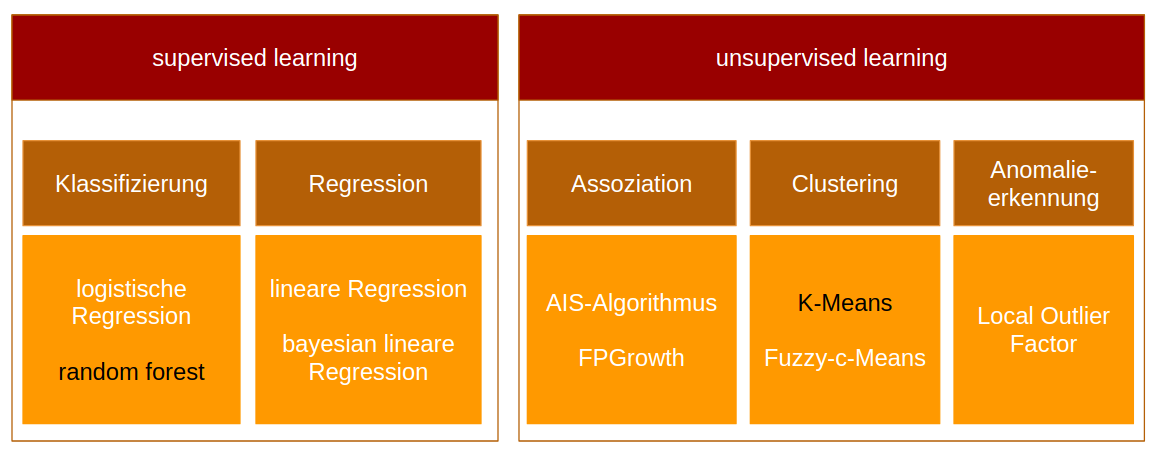
\includegraphics[width=1\textwidth]{verfahren.png}
		\caption{Übersicht der Verfahren (Quelle: Eigenkreation)}
\end{figure}

\section{Supervised Learning}
Beim supervised Learning (zu deutsch: überwachtes Lernen), sind die Zielwerte bekannt. Diese sind entweder aufgrund von Naturgestzen oder Expertenwissen gegeben. Ziel dieser Vorgehen ist es, einen Eingabewert einer dieser bekannten Zielwerte zuzuweisen.

\subsection{Klassifikationsverfahren}
\begin{figure}[h!]
	\centering
	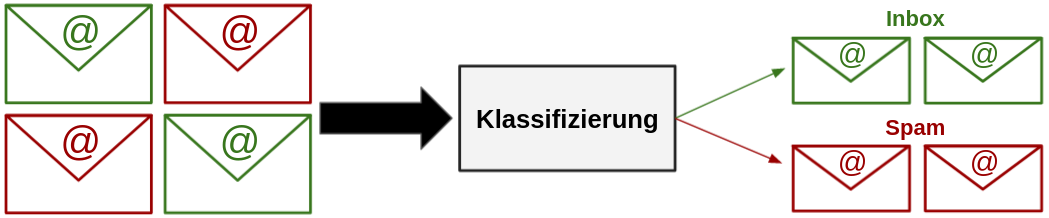
\includegraphics[width=1\textwidth]{classification.png}
	\caption{Klassifizierung von E-Mails (Quelle: Eigenkreation)}
\end{figure}
Bei der Klassifikation geht es darum, einen Datensatz einer Klasse aus einem gegeben Klassenpool zuzuweisen. Das einfachste Beispiel einer Klassifikation ist das erkennen von Spam-Mail. Hierbei haben wir den Klassenpool (Spam, nicht-Spam). Ein eigehendes Mail wird nun entweder der Klasse Spam oder der Klasse Nicht-Spam zugewiesen. Der Algorithmus, welcher diese Zuteilung macht, nennt sich Klassifikator.
Beim Mailbeispiel sprechen wir von einer binären Klassifikation, da wir genau zwei Klassen in unserem Klassenpool haben. Dem gegenüber steht die Multiklassenklassifizierung, bei der mehr als zwei Klassen im Klassenpool bestehen. Ein Beispiel hierzu ist die Klassifizierung von Früchten in die Klassen (Apfel, Birne, Orange, Aprikose).
Zu beachten gibt es hierbei, dass mit der Anzahl Klassen auch die Schwierigkeit der korrekten Klassifikation anwächst. Deshalb ist häufig eine binäre Klassifikation einer Multiklassenklassifizierung vorzuziehen, sofern sich das Problem entsprechend vereinfachen lässt.

Beispiele von Klassifikationsverfahren sind die logistische Regression oder Random Forest.

\subsection{Regressionsanalyse}
\begin{figure}[h!]
	\centering
	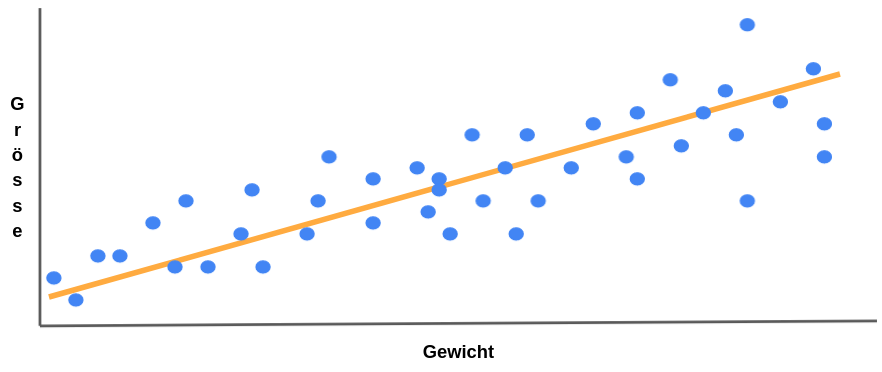
\includegraphics[width=1\textwidth]{regression.png}
	\caption{Bestimmung der Grösse durch Gewicht (Quelle: Eigenkreation)}
\end{figure}
Bei der Regressionsanlyse wird versucht, mittels einer abhängigen und einer oder mehreren unabhängigen Variablen ein Zusammenhang zu modellieren. Wichtig ist dabei die Abhängigkeit der ersten Variable. Fehlt diese funktioniert die Regression nicht. So ist es als Beispiel möglich, mittels Regression das Gewicht eines Menschen anhand seiner Körpergrösse zu modellieren, da grössere Menschen eher ein höheres Gewicht vorweisen. Jedoch ist es nicht möglich, aufgrund der Körpergrösse eines Menschen sein Jahreseinkommen vorauszusagen, da die beiden Variabeln unabhängig voneinander sind.
Eine einfache und häufige Art ist die lineare Regression. Hierbei wird versucht eine Funktion zu finden, die den Zusammenhang zwischen den variabeln möglichst genau beschreibt. Bei einer Einflüssgrösse (z. B. der Körpergrösse) und einer Zielgrösse (z. B. dem Gewicht), führt dies zu einer linearen Funktion.
Diese Funktion kann auf verschiedene Arten berechnet werden. Eine gängige Möglichkeit bildet hier die Methode der kleinsten quadratischen Abweichung. Dabei wird die lineare Funktion gesucht, welche zu allen gegebenen Datenpunkten die kleinst mögliche quadratische Abweichung erzielt.

Ein weiteres Beispiel für die Regression ist die bayesian lineare Regression.

\section{Unsupervised Learning}
Beim unsupervised learning (zu deutsch: unüberwachtes Lernen) sind im Gegensatz zum supervised learning die Zielwerte nicht bekannt. Bei diesen Verfahren wird versucht innerhalb der Daten Muster zu erkennen, damit neue Erkentnisse aus den Daten gezogen werden können.


\subsection{Assoziationsanalyse}
\begin{figure}[h!]
	\centering
	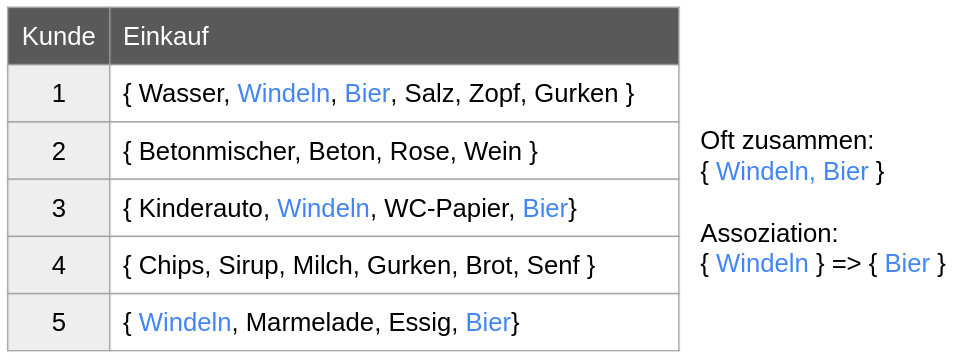
\includegraphics[width=1\textwidth]{association.png}
	\caption{Warenkorbanalyse (Quelle: Eigenkreation)}
\end{figure}
Bei der Assoziationsanalyse wird versucht eine Korrelation zwischen gemeinsam auftrettenden Items herzustellen.
Ein Item ist dabei ein Element einer gegebenen Menge. Durch Assoziation soll also herausgefunden werden, welche Items häufig gemeinsam auftretten. Ein häufiges Beispiel dazu ist die Analyse von Warenkörben. Dort wird versucht herauszufinden, welche Produkte häufig miteinander gekauft werden. So wurde als Beispiel herausgefunden, dass Männer zwischen 30 und 40 Jahre am Samstag häufig Windeln und Bier zusammen kaufen.

Zwei Beispiele für die Assoziationsanylse sind der AIS-Algorithmus und FPGrowth.

\subsection{Clusteranalyse}
\label{sec:clustering}
\begin{figure}[h!]
	\centering
	\includegraphics[width=1\textwidth]{clustering.png}
	\caption{Gruppieren durch Alter und Einkommen (Quelle: Eigenkreation)}
\end{figure}
Bei der CLusteranalyse geht es darum, Daten in verschiedene Gruppen einzuteilen. Das Ziel ist, dass jede Gruppe Elemente beinhaltet, die sich möglichst ähnlich sind. Inwiefer sich die Elemente ähnlich sind, spielt dabei für die Clusteranalyse keine Rolle. So kann die Ähnlichkeit bei Personendaten zum Beispiel aufgrund des Einkommens entstehen oder auch aufgrund der Herkunft der Personen. Auch eine Einteilung nach Alter wäre in so einem Falle denkbar. Wie die Ähnlichkeit bestimmt wird, hängt also davon ab, welche Daten (z. B. nur das Einkommen oder nur das Geschlecht) wir dem Algorithmus liefern.

Deshalb sind diese Gruppen am Anfang noch nicht zwangsläufig bekannt und werden erst durch die Analyse bestimmt. Sobald die Gruppen generiert wurden, kann untersucht werden welches die bestimmenden Merkmale einer Gruppe sind. Dies kann der Algorithmus nicht selber interpretieren. Die Interpretation der Gruppen ist ein seperater, oft manueller Schritt im Prozess. Hier sind allemvoran auch die Gruppen spannend, die wir nicht erwartet haben, da durch diese neue Informationen gewonnen werden. 

Oft verwendete Verfahren sind hierbei der K-Means-Algorithmus und der Fuzzy-c-Means-Algorithmus.

\subsection{Anomalieerkennung}
\begin{figure}[h!]
	\centering
	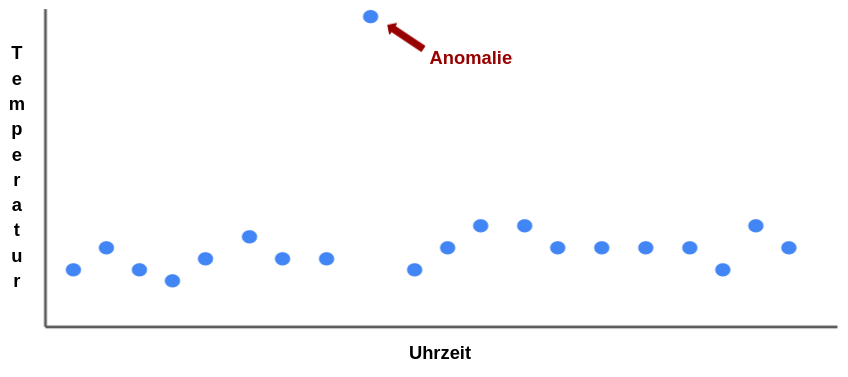
\includegraphics[width=1\textwidth]{anomanlie.png}
	\caption{Falsche Werte erkennen bei Wetterstation (Quelle: Eigenkreation)}
\end{figure}
Die Anomalieerkennung wird verwendet um zu erkennen, welche Datensätze nicht in ein bekanntes Muster passen. Es wird also konkret nach Ausreissern gesucht. Ein Beispiel hierzu sind Kreditkartendaten. Bei einer Kundin die normalerweise jeweils Beträge zwischen 50 und 200 Franken bezieht, wäre ein Bezug von mehreren Tausend Franken ein Ausreisser. Hierbei könnte es sich um eine betrügerische Aktion handeln. So könnte in diesem Beispiel durch den Ausreisser der Diebstahl der Karte festgestellt werden.
Ein weiteres Beispiel kann sein, Fehler in den Datenbeständen zu identifizieren. Eine Temperaturmessstation, die meist Werte zwischen 0 und 20 Grad liefert weisst wahrscheinlich eine Fehlfunktion auf, sollte sie einen Wert von 50 Grad liefern. Durch die Anomalieerkennung können solche Fehler ebenfalls schnell gefunden werden.

Ein bekannter Algorithums für diese Erkennung ist der Local Outlier Factor.


\chapter{Beispiele von Verfahren}

\section{k means}
\section{Random Forrest}

\chapter{Fazit}

\section{Diskussion}
\section{Erkentnisse}
\section{Ausblick}


% Bibliography (Literaturverzeichnis)
\printbibliography

% Inhaltsverzeichnis
\phantomsection 
\addcontentsline{toc}{chapter}{\listfigurename} 
\listoffigures

% Eidesstattliche Erklärung
\chapter*{Erklärung zur Autorenschaft\markboth{Erklärung zur Autorenschaft}{}}
% Append to list of contents
\addcontentsline{toc}{chapter}{Erklärung zur Autorenschaft}




Ich erkläre hiermit, dass es sich bei der eingereichten Arbeit um meine eigene, selbständige Arbeit handelt. Alle direkt oder indirekt verwendeten Quellen sind als Referenzen angegeben. 
\\
\\
Diese Arbeit wurde bisher noch keinem anderen Prüfungsausschuss vorgelegt und ist nicht veröffentlicht worden.
\\
\\
Mir ist bekannt, dass eine falsche Angabe der Autorenschaft rechtliche Konsequenzen nach sich ziehen kann. 

\vspace*{1.5cm} \par
\line(1,0){200} \par
\docLocationFH, \docHandOverDate ~~\docPrenameA~\docSurnameA

% Zurücksetzen \chaptermark
\let\chaptermark\oldchaptermark

% Einbindung des Anhangs
% Hier können Anhaenge angefuegt werden

\begin{appendices}

\end{appendices}
\end{document}      